\section{Durchführung}
\label{sec:Durchführung}
Zu erst wird das Termoelement und somit das Kalorimeter geeicht indem
beide Enden des Thermoelements in Eiswasser gelegt wird. Die nun vom Digitalvoltmeter
abzulesende Spannung die sich zwischen den Enden des Thermoelements ergibt, wird
als Referenzspannung für $T = 0 \si{\celsius}$ angenommen.
Dann wird die Methode zur Bestimmung von $c_gm_g$ aus Kapitel \ref{sec:Theorie}
verwendet, indem zwei Wassermengen abgemessen werden und eine davon zum Kochen
gebracht wird. Danach werden beide Mengen vermischt und die Mischungstemperatur
gemessen. Wichtig dabei ist mit der Messung zuwarten bis sich eine konstante
Mischungstemperatur eingestellt hat. Danach werden die Proben in kochendem
Wasser erhitzt. Im Kalorimetergefäß wird eine Menge Wasser eingefüllt und die
Temperatur gemessen. Danach wird die erhitzte Probe in das Kalorimetergefäß
eingeführt und die Mischungstemperatur bestimmt.
Der Vorgang wird für Graphit und Blei dreimal wiederholt.  Danach wird noch eine
Messung für ein beliebiges Material durchgeführt, in unserem Fall für Kupfer.
Eine Skizze des Versuchsaufbau ist in Abbildung \ref{fig:skizze} zusehen.

\begin{figure}
  \centering
  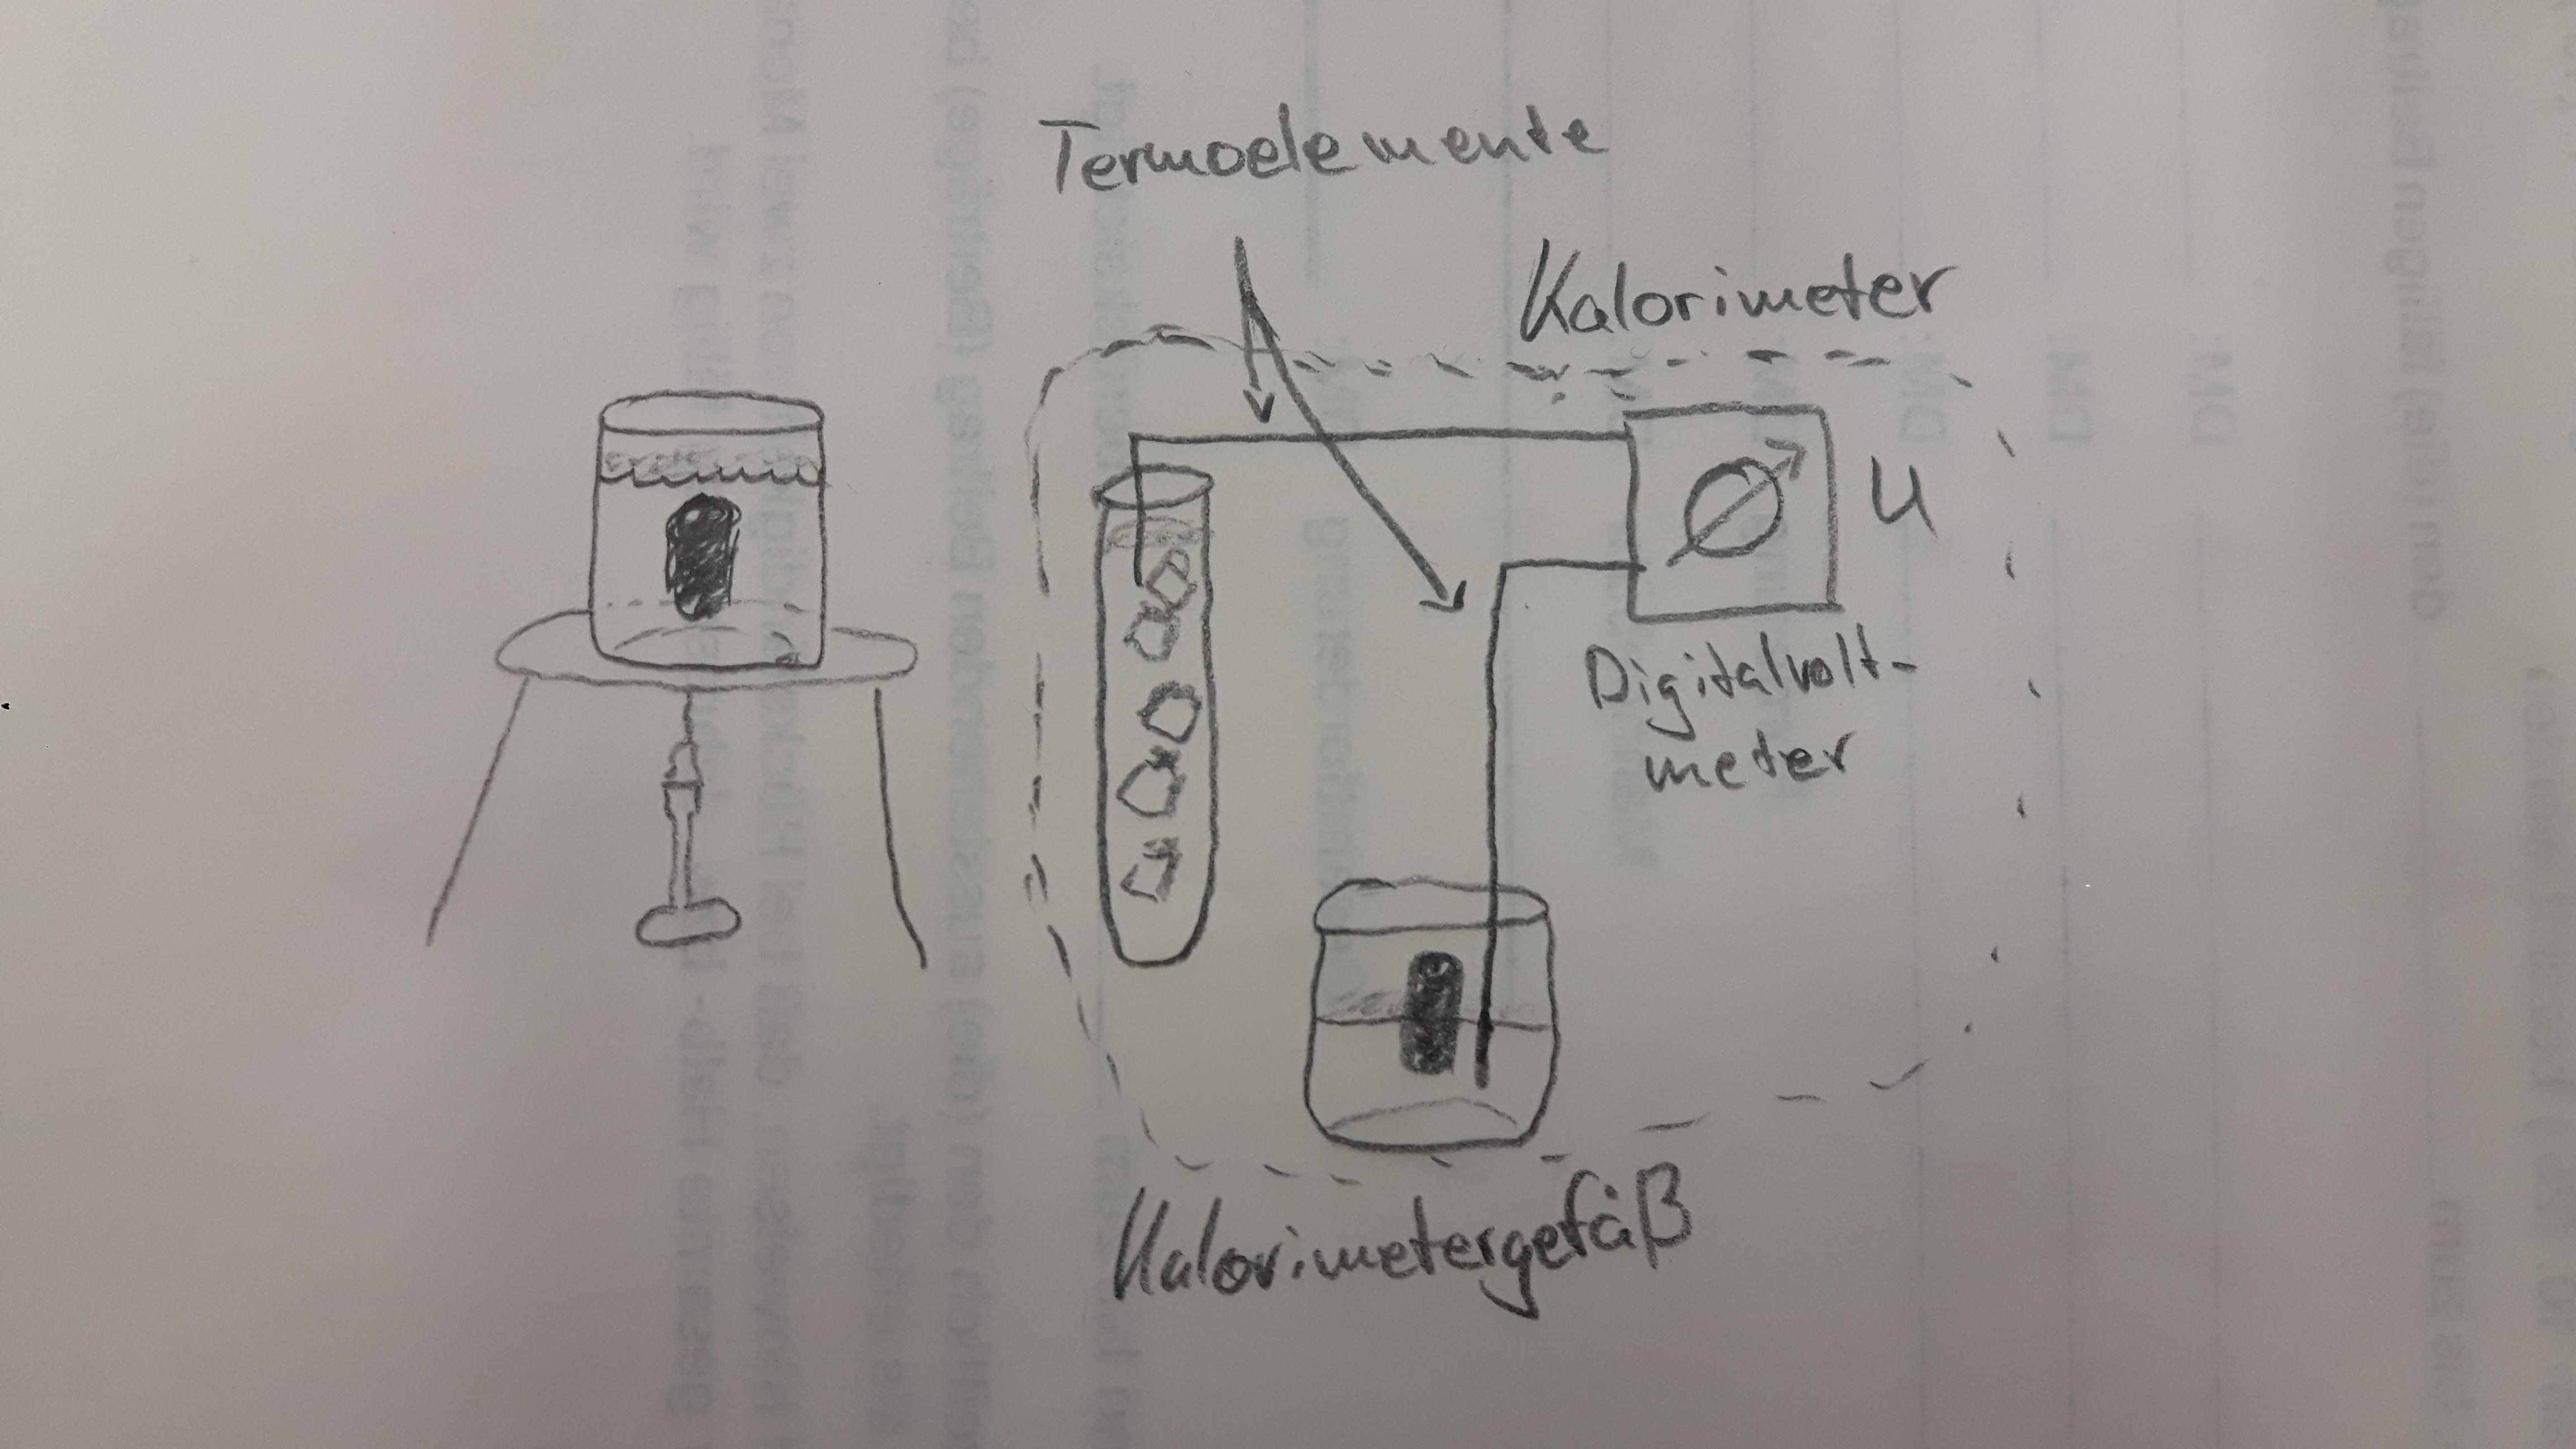
\includegraphics[height=5cm]{logos/skizze.jpg}
  \caption{Schematische Abbildung der Messapparatur}
  \label{fig:skizze}
\end{figure}
